% To familiarize yourself with this template, the body contains
% some examples of its use.  Look them over.  Then you can
% run LaTeX on this file.  After you have LaTeXed this file then
% you can look over the result either by printing it out with
% dvips or using xdvi.
%

\documentclass[twoside,english]{article}
\setlength{\oddsidemargin}{0.25 in}
\setlength{\evensidemargin}{-0.25 in}
\setlength{\topmargin}{-0.6 in}
\setlength{\textwidth}{6.5 in}
\setlength{\textheight}{8.5 in}
\setlength{\headsep}{0.75 in}
\setlength{\parindent}{0 in}
\setlength{\parskip}{0.1 in}

%
% ADD PACKAGES here:
%

\usepackage{amsmath,amsfonts,graphicx,algorithm,caption}
\usepackage[noend]{algpseudocode}
\usepackage{hyperref}
\usepackage{natbib}
\usepackage[document]{ragged2e}
\usepackage{graphicx} %package to manage images
\usepackage{amsmath}
\usepackage{mathtools}
%
% The following commands set up the lecnum (lecture number)
% counter and make various numbering schemes work relative
% to the lecture number.
%
\newcounter{lecnum}
\renewcommand{\thepage}{\arabic{page}}
\renewcommand{\thesection}{\arabic{section}}
\renewcommand{\theequation}{\arabic{equation}}
\renewcommand{\thefigure}{\arabic{figure}}
\renewcommand{\thetable}{\arabic{table}}
\makeatletter
\def\BState{\State\hskip-\ALG@thistlm}
\makeatother
%
% The following macro is used to generate the header.
%
\newcommand{\lecture}[4]{
   \pagestyle{myheadings}
   \thispagestyle{plain}
   \newpage
   %\setcounter{lecnum}{#1}
   \setcounter{page}{1}
   \noindent
   \begin{center}
   \framebox{
      \vbox{\vspace{2mm}
    \hbox to 6.28in { {\bf IE 506: Machine Learning - Principles and Techniques
		\hfill Jan-May 2023} }
       \vspace{4mm}
       \hbox to 6.28in { {\Large \hfill End-term Project Report : #1  \hfill} }
       \vspace{2mm}
       \vspace{2mm}
       \hbox to 6.28in { {\it Team Name: #2 \hfill Team Members: #3} }
       %\vspace{2mm}}
       %\hbox to 6.28in { {\it Due Date: 01-August-2018} }
      \vspace{2mm}}
   }
   \end{center}
%   \markboth{Assignment #1: #2}{Assignment #1: #2}

   %{\bf Note}: {\it LaTeX template courtesy of UC Berkeley EECS dept.}

   %{\bf Disclaimer}: {\it These notes have not been subjected to the
   %usual scrutiny reserved for formal publications.  They may be distributed
   %outside this class only with the permission of the Instructor.}
   \vspace*{4mm}
}
%
% Convention for citations is authors' initials followed by the year.
% For example, to cite a paper by Leighton and Maggs you would type
% \cite{LM89}, and to cite a paper by Strassen you would type \cite{S69}.
% (To avoid bibliography problems, for now we redefine the \cite command.)
% Also commands that create a suitable format for the reference list.
\renewcommand{\cite}[1]{[#1]}
\def\beginrefs{\begin{list}%
        {[\arabic{equation}]}{\usecounter{equation}
         \setlength{\leftmargin}{2.0truecm}\setlength{\labelsep}{0.4truecm}%
         \setlength{\labelwidth}{1.6truecm}}}
\def\endrefs{\end{list}}
\def\bibentry#1{\item[\hbox{[#1]}]}

%Use this command for a figure; it puts a figure in wherever you want it.
%usage: \fig{NUMBER}{SPACE-IN-INCHES}{CAPTION}
\newcommand{\fig}[3]{
			\vspace{#2}
			\begin{center}
			Figure #1:~#3
			\end{center}
	}
% Use these for theorems, lemmas, proofs, etc.
\newtheorem{theorem}{Theorem}[lecnum]
\newtheorem{lemma}[theorem]{Lemma}
\newtheorem{proposition}[theorem]{Proposition}
\newtheorem{claim}[theorem]{Claim}
\newtheorem{corollary}[theorem]{Corollary}
\newtheorem{definition}[theorem]{Definition}
\newenvironment{proof}{{\bf Proof:}}{\hfill\rule{2mm}{2mm}}

% **** IF YOU WANT TO DEFINE ADDITIONAL MACROS FOR YOURSELF, PUT THEM HERE:
\newcommand{\R}{\mathbb{R}}

\begin{document}
%FILL IN THE RIGHT INFO.
%\lecture{**LECTURE-NUMBER**}{**DATE**}{**LECTURER**}{**SCRIBE**}
\lecture{Creating Graphics Programs from Images}{Your team's name}{Roll numbers of team members}
%\footnotetext{These notes are partially based on those of Nigel Mansell.}

% **** YOUR NOTES GO HERE:

% Some general latex examples and examples making use of the
% macros follow.  
%**** IN GENERAL, BE BRIEF. LONG SCRIBE NOTES, NO MATTER HOW WELL WRITTEN,
%**** ARE NEVER READ BY ANYBODY.

\begin{abstract}
	This project report contains the details on our project which aims to infer graphics software programs from hand-drawn images. We describe the deep learning tools involved in our project. In particular, we explain about the ML method used for the project, the details of training procedure, details of inference and discuss about experiments conducted. We have tried a new ML method and superior results are presented using the proposed method.
\end{abstract}

\section{Introduction}

Provide a short introduction about the project with proper motivation and applications. Give a broad overview of the project without getting much into the details. 

Explain the structure of the project report as below:

We provide a survey of existing literature in Section \ref{sec:litsurvey}. Our proposal for the project is described in Section \ref{sec:our_proj}. We give details on experiments in Section \ref{sec:exp}. A description of future work is given in Section \ref{sec:future_work}. We conclude with a short summary and pointers to forthcoming work in Section \ref{sec:conclusion}.

\section{Literature Survey} \label{sec:litsurvey}

Explain at least 3 to 5 previous works relevant to your project. Cite the required papers. See the following example.

Our project draws inspiration from a closely related work by Ellis et al. \citep{paper}. In their paper \citep{paper}, the authors describe a three-step process where an input hand-drawn image is first used to generate a program specification (spec) which is then used to generate a graphics software program which is later rendered to generate the hand-drawn image as a graphics object (like a bitmap image, jpeg image, etc.).  This process is illustrated in Figure \ref{threestepprocimg}.

\begin{figure}[!h]
	\centering
	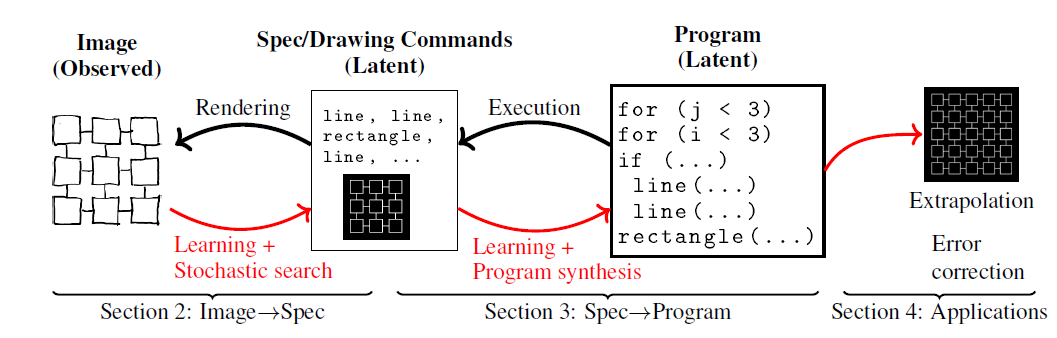
\includegraphics[scale=0.8]{threestepprocess}
	\caption{Three Step Process to generate program specs from image and then to convert specs to graphics programs and later render the programs to graphics objects}\label{threestepprocimg}
\end{figure}


  
 A few experiments on a dataset are provided which indicate the usefulness of the approach.


\section{Methods and Approaches} \label{sec:our_proj}

Give details on the proposed project. Explain how it is different from existing work. Explain the ML method to be used. Explain all other required details.

\subsection{Work done before mid-term project review} 
This section can be populated from your mid-term project report. 

\subsection{Work done after mid-term project review} 

Give details on the work done after the mid-term project review. Explain how it is significant. Explain the ML method used and changes you tried. Explain all other required details.

\section{Data set Details} \label{sec:data}

Explain all details  on the data sets used for the project. Description of data size and attributes, nature and type of data (image/audio/text/video etc.), data pre-processing techniques used should be illustrated. Other relevant details on data procurement (the website from where the data is obtained), and how the data is to be used in experiments should be described. 

\section{Experiments} \label{sec:exp}

Give details on experiments performed. Training procedure and algorithm, the settings used for optimization algorithm and other relevant algorithmic details need to be included. Details on the hardware configuration should also be described. 

\section{Results}\label{sec:results}

Add suitable plots and tables describing the results obtained during the project. Comparative results should be included if new ideas are tried. Description of the results and the inferences made using the results should be described. 

\section{Future Work} \label{sec:future_work}

Explain the work to be done further. 

\section{Conclusion} \label{sec:conclusion}

Conclude by giving a summary of your project, summarizing the problem, the methods used, and the significance of results obtained. Give some indications of future work to be done. 

\bibliographystyle{plain}
\bibliography{demo} % Because the file name is demo.bib


\end{document}

